%%% Local Variables:
%%% mode: latex
%%% TeX-master: "../index"
%%% End:

% Recommended:
% Explain with AES (not an requirement)
% Why do we chain blocks?
% Do example with matrix
% CBC-MAC

\subsection*{Agenda}
\begin{enumerate}
\item Block ciphers
\item AES
\item Modes of operation
\item CBC-MAC
\end{enumerate}

\subsection{Block ciphers}

Symmetric key cipher. ``Pseudo Random Permutations'', they scramble a
plaintext $m$ using a key $k$ to produce a seemingly random text
$c$. Can be reversed using the same key $k$.

\subsubsection*{Security goal of block ciphers}

The ciphertext should be indistinguishable from a truly random text,
so an adversary cannot tell whether a given text is an encryption or
random.

\subsection{AES}
Block size $128$ bits, key size $128, 192$ or $256$ bits

\subsubsection*{AES algorithm outline}

\begin{enumerate}
\item AddRoundKey
\item Repeat 9 times
  \begin{enumerate}
  \item SubBytes
  \item ShiftRows
  \item MixColumns
  \item AddRoundKey
  \end{enumerate}
\item SubBytes
\item ShiftRows
\item AddRoundKey
\end{enumerate}

\subsubsection{MixColumn operation}
Mixes column values using matrix multiplication
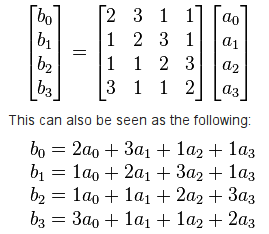
\includegraphics[scale=0.6]{images/4-mixcol}

\subsection{Modes of operation}

\subsubsection*{Electronic Code Book}

All blocks encrypted independantly from each other.

\textbf{Disadvantages:} Equal message blocks gives equal cipher
blocks, length of $m$. Attacker can permute blocks and will decipher
to a valid message.

\subsubsection*{Cipher Block Chaining}

Encryption of block $m_i$ depends on cipher block $c_{i-1}$. An
\texttt{IV} (Initialization Vector) is used as the first dependency.

\begin{align*}
  c_i = e_k(m_i \oplus c_{i - 1})\\
  m_i = d_k(c_i) \oplus c_{i-1}
\end{align*}

\textbf{Disadvantages:} lost or tampered transmission of one block
results in wrong decryption of full plaintext

If block size does not divide messages length, the length is padded.

\subsection{CBC-MAC}

Message authentication code using block ciphers (for instance
AES). Given text blocks $x_1, \ldots, x_t$ of $n$ bits

Forgery attack

Given $m$ and $t = MAC_K(m)$, and $m'$ and $t' = MAC_K(m')$, one can forge a message $m''$ by

\[ m || m'_1 \oplus t || m'_2 || \ldots \]

Because $m'_1 \oplus t$ will cancel the contribution of the first MAC, making $MAC_K(m'') = t'$

\subsubsection{Prevent attack}
\begin{itemize}
\item Prepend length of message in the first block
\item Encrypt last block with $K_2$
\end{itemize}

\subsubsection{Padding rule}
